% example.tex - an example workterm report that can be used as a template for writing NE
% workterm reports

% We begin by calling the workreport class which includes all the definitions for the macros
% and environments we will be using throughout the document.
\documentclass{workreport}

% We will use some packages to add some functionality to our script.
% The lipsum package is only used to create placeholder text for this example. It can be
% deleted when your own text has been filled into the sections.
\usepackage{lipsum}
% The amsmath package provides various features to facilitate writing math formulas.
\usepackage{amsmath}
\usepackage{subcaption}


% LaTeX also supports file splitting between documents. For example, your
% introduction section could be in its own "introduction.tex" file, and you
% can import it here. This is normally done with the \input command.

% The \addbibresource command finds a BiBLaTeX file, and adds it to the
% document. BiBLatex and BiBTex are TeX extensions that automatically build
% format citations and references based on a key-value database sitting in a
% text file. In our case, this file is example.bib. We add this to the preamble
% (the part of the tex file before \begin{document}) here.
\addbibresource{./example.bib}


%%%%%%%%%%%%%%%%%%
%  IMPORTANT  INFORMATION  %
%%%%%%%%%%%%%%%%%%

% Fill in the title of your report
\title{
	Design of Bluetooth Low Energy Controlled Model Rocket
}

% Fill in your name
\author{Tong Wu}

% Fill in your student number
\studentnumber{20470965}

% Fill in your student ID
\studentid{t53wu}

% Fill in your previous academic term
\previousterm{3B}

% Fill in the name of your university
\university{University of Waterloo}

% Fill in your faculty
\faculty{Engineering}

% Fill in your program
\program{Nanotechnology Engineering}

% Fill in your program director
\programdirector{Shirley Tang}

% Fill in the address of your university
\universityaddress{
	200 University Ave. West \\
	Waterloo, ON \\
	N2L 3G1
}

% Fill in your employers name
\employername{Nordic Semiconductor ASA}

% Fill in your employers address
\employeraddress{
	Otto Nielsens veg 12, \\
	7052 Trondheim
}

% We will now begin writing the document
\begin{document}

%%%%%%%%%%%
% FRONT MATTER %
%%%%%%%%%%%

% The \begin{frontmatter} command will allow the use of the following environments:
% letter_of_submittal, contributions, summary, conclusions, recommendations, toctree
% (table of contents) and listoffiguresandtables (list of figures and list of tables).
\begin{frontmatter}

% The letter_of_submittal environment requires two inputs, the first being the greeting
% and the second being the closing.
\begin{letter_of_submittal}{Dear Dr. Tang:}{Sincerely,}

	% You're letter body.
	This work report, titled “Design of Bluetooth Low Energy Controlled Model Rocket”, was written upon the completion of my 3B work term for Nordic Semiconductor ASA. This report is to be submitted for the fulfillment of WKRPT 400. The purpose of the report is to reflect on the engineering design process behind the model rocket demo project for the Applications Group and to pass on knowledge of model rocketry to the rest of the group so that the project can be further developed and improved upon if desired.

	Nordic Semiconductor ASA is a Norwegian technology company that focuses on delivering the best ultra-low power wireless solutions and is currently a leader in the Bluetooth Low Energy market. The company's profit source is the selling of Bluetooth Low Energy chips, but it also has many teams that work on relevant hardware, software, and services which are provided to their customers or potential customers free of charge in order to help them easily integrate Nordic chips into their products and business. During my work term I worked in the Applications Group, led by Endre Rindalsholt, which is mainly responsible for creating reference designs and demo projects to showcase potential product concepts and a sample design for customers to reference their products off of.

	I hereby confirm that I have received no assistance in writing this report. I also confirm this report has not been previously submitted for academic credit at this or any other academic institution.


\end{letter_of_submittal}

% The contribution environment only requires the contributions text.
\begin{contributions}

  During my employment at the Applications Group, the team consisted of around 15 full-time employees and summer students working on embedded firmware, electrical hardware, and web applications for Bluetooth Low Energy devices. These projects were all aimed to help our customers have a easier time developing products with our chips and help them reach full volume production and go to market faster. It was a very energetic group with lots of exciting multidisciplinary hands-on projects.

	My three projects at Nordic were sensor driver development, security enhanced Eddystone beacon firmware development in partnership with Google, and finally a Bluetooth Low Energy (BLE) enabled model rocket demo project. The project that will be reported on and discussed in detail in the report is the BLE enabled model rocket. The purpose of this project was to create a proof of concept (PoC) prototype of a model rocket that is running on Nordic's latest BLE system-on-chip (SoC), nRF52832, to showcase an application of BLE in medium-range toys because future BLE specifications are going to allow for higher transmit powers thus significantly increasing the previously limited range of BLE and making it a suitable technology for medium range applications. Moreover, this project was an opportunity for me to develop my skills in printed circuit board (PCB) layout and schematic design, antenna tuning, and mechanical design which were laid out as part of my learning outcomes in the beginning of the work term. The entire process involved internet research of the current model rocketry market, the existing types of model rockets and their associated flight dynamics and equipment requirements and instruments, as well as available purchasing locations for such resources; prototyping of a reliable engine ignition mechanic and parachute deployment mechanic; circuit design and PCB layout of the entire electronic system including the communication system, telemetry system, and ignition and recovery deployment system; design and prototype the mechanical assembly through 3D modeling and 3D printing, and finally validation and tuning of flight dynamics with model rocketry simulation software. This project was mainly a solo effort with input and constructive feedback from my teammates on specific topics of their expertise such as firmware and electronics.

	The relationship between this report and my work is that the report captures all the new knowledge developed about electronic wireless model rocketry which is a brand new field of knowledge in the group. Also this report allows me to reflect on the engineering design and analysis behind several complex systems in the rocket which all manifest into very useful lessons for my future career. It also serves as a reminder that any technical knowledge, even rocket science, can be learned from the ground up in a shot span of time as long as you put your curious and analytical mind behind it!

	In the broader scheme of things, my work at Nordic Semiconductor on the BLE model rocket project has set an example that broadens the horizon on what kind of applications BLE can be at the heart of. It pushes the boundaries on what kind of devices people typically associate with BLE and have also generated significant social media interest for Nordic Semiconductor by live broadcasting the rocket launch on Facebook, thusly creating a cool and fun image for the company. My work with the rocket has also introduced many members of the team to a cloud-based 3D modeling software, OnShape, that I have picked up from my previous work term that is much more powerful and easier to use than the then status quo in the office, SketchUp. And most importantly it got many team members and their children interested in model rocketry which actually fulfills one of the main missions of the model rocketry industry, to stimulate interest in the wider public about science and engineering through this exciting hobby.

\end{contributions}

% The summary environment only requires the summary text.
\begin{summary}

	The main purpose of the report is to summarize and communicate the research and development done on the BLE model rocket project in my work term at Nordic Semiconductor ASA in Trondheim, Norway. This report will communicate the motivation and significance of the project that I had worked on and also record the engineering analysis and design that went into this work. The scope of this work includes the background research done in model rocketry, the different design options considered for the prototype, the construction requirements for launch, and several recommendations for future revisions of the rocket.

	The major points documented in this report are the entire design and prototyping phases of the model rocket and the recorded details where are important to the successful ignition, flight, and recovery of the rocket. Also, sufficient background in model rocketry and BLE electronics is provided in order to give insight to some of the related design decisions related to those fields.

	The major conclusions documented in this report are that using BLE to remotely control the launch of a model rocket is more versatile, convenient, and safe than traditional methods of a wired ignition box; that a BLE chip coupled with power amplifier can easily achieve a communication range of more than 200 meters if the antenna is properly tuned; and that real-time telemetry data from the rocket is an insightful metric into the flight performance of the rocket.

	The major recommendations of this report are that the exhaust end of the rocket should be sufficiently lifted from ground to avoid undesired ignition of adjacent engines in a multistage launch; that the parachute deployment system should be rocket-body-orientation-agnostic; and that flight data should be internally logged into the random access memory (RAM) of the BLE chip as well as communicated over the air in case the rocket travels out of range, so that the data can be read back after retrieval of the rocket.


\end{summary}

% The conclusions environment only requires the conclusions text.
\begin{conclusions}



\end{conclusions}

% The recommendations environment only requires the recommendations text.
\begin{recommendations}

        \lipsum[1-3]

\end{recommendations}

% The following command generates a table of contents (toc) that automatically keeps
% track of sections and their page numbers.
\toctree

% The following command generates a list of figures and a list of tables that
% automatically keep track of properly inserted figures and tables. The commands for
% properly inserting figures and tables will be explained in the body section of this
% document.
\listoffiguresandtables

\end{frontmatter}

% The \newglossaryentry{title} command creates an entry for the glossary. It requires a
% name and description. The title is used for making references to the glossary entry
% throughout the document. For more information on the glossary and acronyms, refer
% to the link under Glossary and Acronyms in README.md.
% These can be located anywhere in the document as long as they are declared before any \gls command references them
\newglossaryentry{LaTeX}{
	name={\LaTeX},
	description={A document preparation system used for
		high-quality typesetting. It is most often used
		for medium-to-large technical or scientific documents.
		\LaTeX is not a word processor!
	}
}

\newglossaryentry{Unix}{
	name={Unix},
	description={A multi-user multi-tasking operating system
		developed by Ken Thompson and Dennis Ritchie in the
		1970s, which has inspired many features behind Mac OSX
		and Linux
}
}

%%%%%%
% BODY  %
%%%%%%

% The \begin{body} command will create the body environment. This environment
% includes the formatting required for the body
\begin{body}

% The \section{title} command creates a section in the body of your report. You must
% specify the title of the section as the commands input. These sections headers will
% automatically be added to the table of contents.
\section{Introduction}

	The goal of the project captured in this report is to demonstrate a reference design of a BLE controlled model rocket, which can be launched, recovered, and reused, using Nordic's nRF52832 SoC in order to generate more market interest in utilizing Nordic's products and more importantly to showcase the possibility of deploying BLE in medium range applications in anticipation of the significantly increased range of the next Bluetooth Specification to be released. Despite the fact that, given the time allotted, the end result is a simply a working PoC and far from a polished design ready to be in the market, it is still a highly multidisciplinary and complex project consisting of design considerations in aerodynamics, newtonian mechanics, embedded system design, radio frequency (RF) electronics, and user experience. In addition, recommendations will be provided to fix and improve upon the current design of the rocket to make it more reliable, more performant, and more user friendly.

	In order to understand the design and engineering process behind this report however, a sufficient amount of background knowledge on model rocketry and BLE electronics is required and hence will be provided next.

\section{Background}

	The background sections introduces many important concepts in model rocketry and BLE electronics at a high level with enough details to allow the understanding and appreciation of the work reported herein.

% The \subsection{title} command creates a subsection for the above mentioned
% section. You must specify the title of the section as the commands input. These
% subsection headers will automatically be added to the table of contents, below the
% proper section.

\subsection{Model Rocketry}

	Model rocketry is a popular hobby that originated in the late 1950's, coinciding with the dawn of the space age, as many space enthusiasts were inspired to build their own rockets by the sight of the space boosters carrying the first artificial satellite into space \cite{estes_rocket_tech}. It started as an extremely dangerous hobby as many people were attempting to create their own propellants with unstable chemicals that often resulted in injuries of tragedies. It was not until when Estes Industries was founded in 1958 to mass manufacture solid propellant model rocket engines did the hobby become safe and very popular amongst younger aspiring rocketeers and families \cite{estes_rocket_tech}.

	Popular model rockets today are mainly constructed with safe materials such as cardboard, plastic, and balsa wood, with sizes ranging from 1 foot to 6 feet. They are fueled by single-use rocket motors (note that the terms motor and engine can be used exchangeably) manufactured professionally by companies such as Estes. The rockets typically contain a recovery device such as a parachute to enable gentle landing and recovery for future flights and reuse of the rocket. The rocket can be flown again by simply replacing the used motor with a fresh one. Typical entry-level model rocket components are shown in Figure \ref{fig:rocket_comp} below.

	\begin{figure}[!ht]
		\centering
		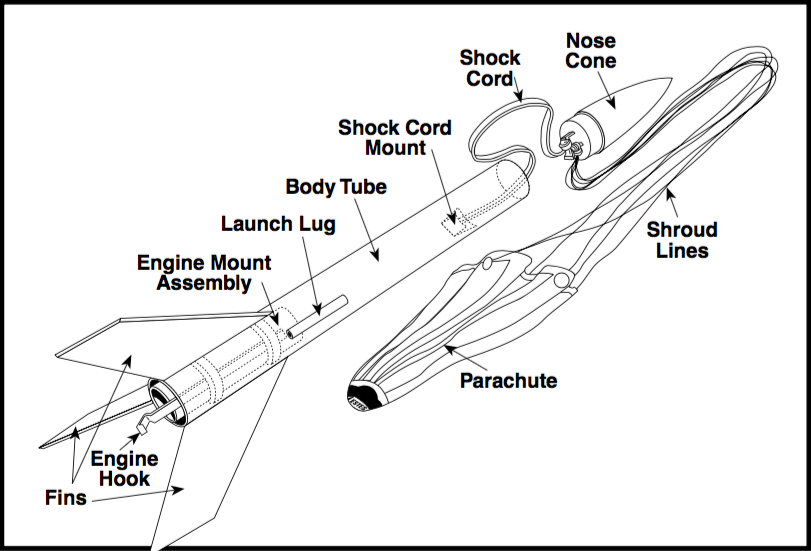
\includegraphics[width=10cm]{./images/model_rocket_components.png}
		\caption{Typical model rocket components - without engine \cite{estes_rocket_tech}}
		\label{fig:rocket_comp}
	\end{figure}


	Typically, a model rocket launch consists of 7 distinct phases: ignition, lift-off, burnout, coasting, apogee, parachute ejection, and soft landing. During ignition, the rocket engine is ignited electrically by a manual switch from a box containing circuits external to the rocket as shown in Figure \ref{fig:ignition_box}.

	\begin{figure}[!ht]
		\centering
		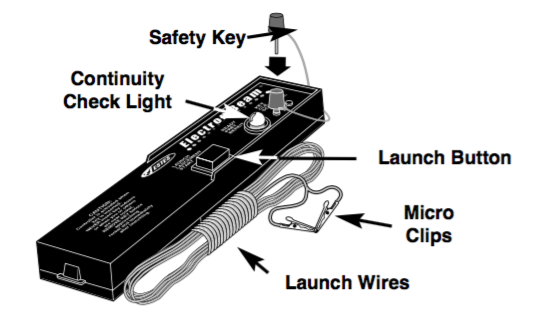
\includegraphics[width=10cm]{./images/ignition_box.png}
		\caption{Ignition Box \cite{estes_rocket_tech}}
		\label{fig:ignition_box}
	\end{figure}

	These boxes work by shorting a battery across the terminals of a motor igniter, which is just a piece of bent wire with some heat sensitive pyrotechnic material at the tip that is inserted into the rocket motor that ignites when heated due to joule heating by the high current passing through the igniter. When the igniter ignites, the combusted pyrotechnic material triggers ignition of the motor propellant and also breaks continuity of the igniter and current should automatically stop flowing. The use of the ignition box is meant to create a safe distance to launch the rocket by using long launch wires with micro clips at the end to attach to the motor igniters. Figure \ref{fig:igniter} shows a schematic of how a motor igniter is installed into the rocket motor.

	\begin{figure}[!ht]
		\centering
		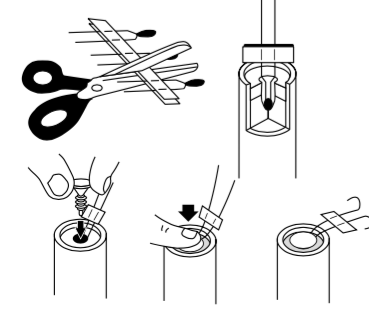
\includegraphics[width=10cm]{./images/igniter.png}
		\caption{Rocket Motor Igniter \cite{estes_rocket_tech}}
		\label{fig:igniter}
	\end{figure}

	However, if a model rocket has embedded electronics inside that can be controlled via a smartphone, then the ignition box can become obsolete and ignition can be performed completely wirelessly from a much longer distance away. This is one of the first design wins for BLE in model rocketry.

	Once the engines are ignited, the rocket will enter the lift-off phase where it accelerates very rapidly off of the launch pad due to the rapid ejection of hot gas (in model rocketry, a launch pad is just a structure that mechanically guides the rocket straight upwards during lift-off). After the rocket leaves the launch pad, it enters the burnout phase where the rest of the propulsion fuel is gradually ejected from the engine and rocket's upward acceleration starts to diminish. At the point where all the propulsion in the engine is exhausted and the provided thrust and therefore upward acceleration becomes zero, the rocket enters the coasting phase, where gravity and air drag begins to slow down the rocket to zero upward velocity. At the point of zero upward velocity, the rocket has reached its apogee, the highest altitude of its flight. Some point after apogee, parachute ejection should take place, preferably as soon as possible after apogee to prevent the rocket from gaining too much downward velocity due to gravity. After parachute ejection, the rocket will eventually enter the last stage of its flight, soft landing. A summative illustration of typical flight phases taken from the Centuri Model Rocket Designers Manual\cite{centuri_manual} is shown in Figure \ref{fig:flight_phase}.


	\begin{figure}[!ht]
		\centering
		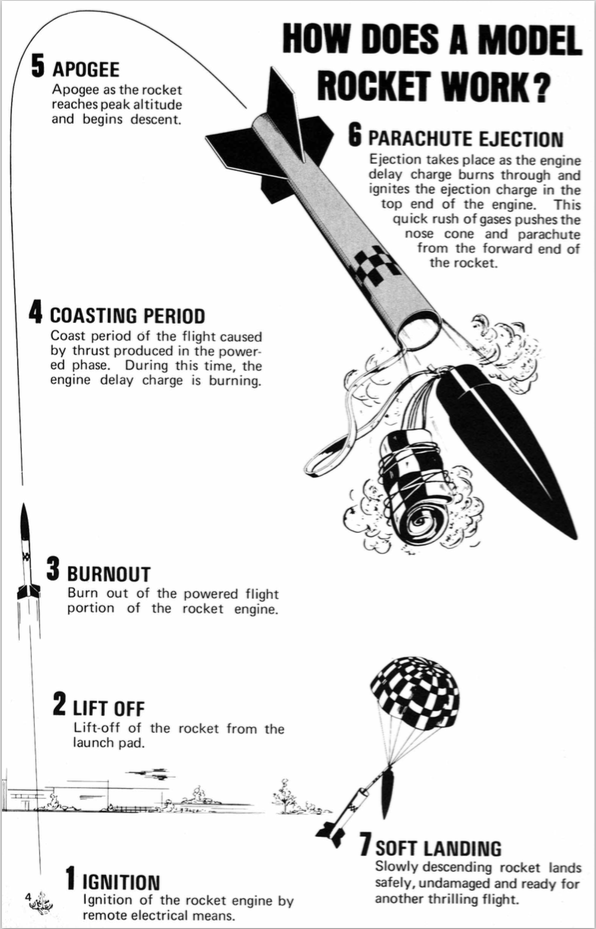
\includegraphics[width=10cm]{./images/flight_phase.png}
		\caption{Model Rocket Flight Phases \cite{centuri_manual}}
		\label{fig:flight_phase}
	\end{figure}

% The \subsubsection{title} command works exactly like the \section{title} and
% \subsection{title} commands above.
\subsubsection{Model Rocketry Engines}

	The engines are the single most important component of any typical model rocket since it is most often responsible for two of the most crucial tasks in rocket flight: provide propulsion and trigger parachute deployment. A visual dissection of a typical model rocket engine is shown in Figure \ref{fig:dissection}. Model rocket engines typically use black powder as solid-fuel to provide thrust to the rocket by rapidly ejecting hot gas out the exhaust end of the engine. After the complete burnout of propulsion material there is a short period of delay charge inside the engine that burns for easier visual tracking but provides no significant thrust to allow the rocket to coast to apogee. Then finally the ejection charge ignites and fills the rocket body tube with hot gas. The sudden increase in pressure in the body tube will pop open the nose cone and push out the parachute assembly. Model rocket engines are categorized with codes indicating their total impulse in newton seconds, average thrust in newtons, and delay charge time in seconds. For model rockets the total impulse range from A to G. This is called the class of the motor. Class A being 0 to 2.5 Ns, and B being 2.6 to 5, with each subsequent class having twice the max allowed total impulse as previous. The average thrust is simply indicated by a number that is the average thrust in newtons, and the delay charge time is also just a number in the number of seconds.
	For example a engine with the code C4-3 means it has a total impulse somewhere from 5.1 to 10 Ns, with an average thrust of 4 Newtons and a delay charge time of 3 seconds. All manufacturers of rocket motors will provided datasheets specifying the exact impulse and thrust curve of their engines.

	\begin{figure}[!ht]
		\centering
		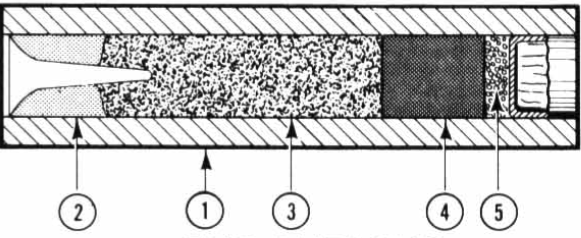
\includegraphics[width=10cm]{./images/dissection.png}
		\caption{Rocket engine dissection \cite{centuri_manual}. 1. Casing 2. Nozzle 3. Propellant 4. Delay Charge 5. Ejection Charge}
		\label{fig:dissection}
	\end{figure}

	The delay charge is designed to allow the rocket to coast in unpowered flight to its apogee before the parachute is ejected with the ejection charge. However each rocket flies differently and the amount of delay charge they need is different depending on their mass and drag. Motor manufacturers make several delay charges available for each motor class. However, that doesn't give the curious users fine grained control for optimization of flight performance. This is where BLE model rockets have another design win over traditional ones: by embedding a BLE module inside the rocket, the parachute can be ejected remotely by command or via intelligent algorithms on-board with altimeter data to determine when the apogee was reached, so it does not have to rely on the limited charge choices made available by the motor manufacturers.

\subsubsection{Model Rocketry Physics}

	The provided overview above of the typical model rocket flight process above sets up the foundation for a general understanding of the sequence of tasks that the BLE model rocket reported in this work must fulfill in order to perform a successful launch. Next it will be very important to provide a background of the physics involved in a successful rocket launch as the mechanical design of the rocket must adhere strictly to the physical guidelines imposed by the laws of aerodynamics and newtonian mechanics in order to ensure a successful flight.

	Like anything that flies, model rokets get airborn by generating enough upward force to overcome gravity and air drag. A model rocket takes flight by utilizing rocket motors which eject gas at high velocities downward out the tail end of the rocket and as a result generating thrust upward (Newton's Second Law). At the most basic level, to overcome gravity, the thrust generated by the motor at lift off must abide by the following equation:

	\begin{align}
		% The following are mathematical equations written using the amsmath
		% package. For more information on writing mathematical equations in
		% LaTeX, refer to the link under AMSMath in README.md.
		\frac{(F_{thrust} - F_{drag})}{Mass_{rocket}} > 9.8 \frac{m}{s^2}
	\end{align}

	Albeit, most engine manufacturers provide a minimum lift-off weight parameter for each engine type to ensure that the user can easily select the correct engine for the rocket. Once the rocket is in the air however, the mathematics become extremely complicated and there are no more simple equations to follow to determine the behaviour of the rocket when it's airborn. To calculate the expected apogee of the rocket and travel time is much more involved since the air drag is a very complicated parameter involving several variables, and that the thrust is time dependent ariable which follows a curve specified by the manufacturer, and that the mass is constantly changing as propellant is constantly being ejected out of the rocket, thus a simulation tool (OpenRocket) will be used to calculate the expected flight trajectory.

	Outside of the simulation tool, the most important factor to for the user to consider in model rocketry is aerodynamic stability. Aerodynamic stability describes a rocket's ability keep its nose pointed in the same direction throughout its upward flight \cite{estes_rocket_tech}. In more technical lanaguage, it is its ability to resist rotation around its center of gravity (CG) while under perturbing forces from factors such as wind or misaligned motor thrust while flying in the air. The two factors above are the main perturbing forces to consider and they are illustrated in Figure \ref{fig:forces}.

	\begin{figure}[!ht]
		\centering
		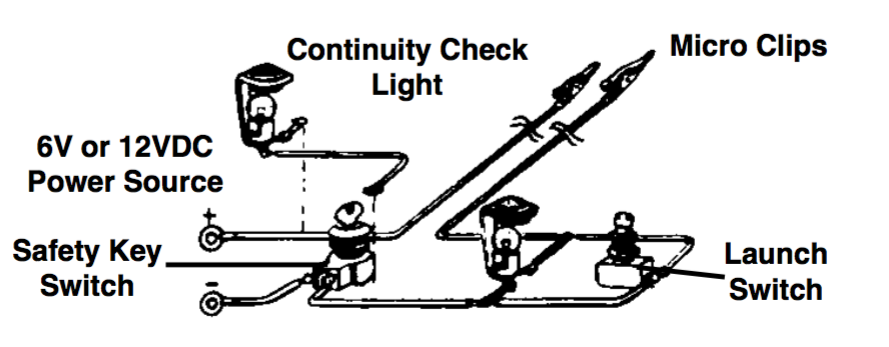
\includegraphics[width=10cm]{./images/forces.png}
		\caption{Perturbing forces on a model rocket}
		\label{fig:forces}
	\end{figure}

	Under perfect conditions with zero wind, the CG and the point of thrust (radial location of the motor) are aligned perfectly at the radial center of the rocket and the rocket would fly straight upwards, provided that it was launched vertically. However, in reality, any small perturbations due to wind or misaligned motor will cause a small (less than 5 degrees) angle of attack (AoA) $\alpha$, and if goes uncorrected, this AOT will become larger and larger which will eventually cause the rocket to tumble uncontrollably in the air and crash into the ground, which is extremely dangerous. To prevent this from happening, fins are untilized on model rockets to provide the stabilizing force. As $\alpha$ increases, the surface area of the fins that are exposed to the oncoming airflow parallel to the flight path increases and the resulting drag on the fins will push back and stabilize the rocket by reducing $\alpha$, as shown in Figure \ref{fig:fin_stable}

	\begin{figure}[!ht]
		\centering
		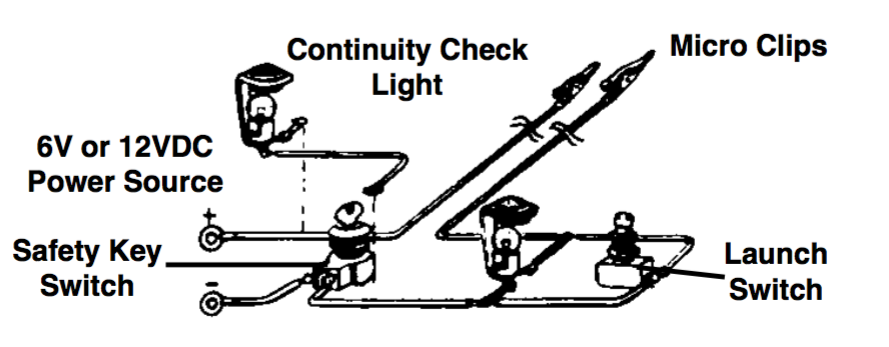
\includegraphics[width=10cm]{./images/fin_stable.png}
		\caption{How fins on model rockets stabilize it in flight}
		\label{fig:fin_stable}
	\end{figure}

	While in the air, the forces perpendicular to the length direction of the rocket can be modeled by a rigid beam on a fulcrum at its CG as shown in Figure \ref{fig:fulcrum}. Another very important point to consider beside the CG is the center of pressure (CP). The center of pressure is the point where all the aerodynamic forces will act through, just like how the gravitational force will act through the center of gravity. And similar to how the location and amount of mass distributed across an object affects the CG, the location and amount of of surface area distributed across an object affects the location of center of pressure.

	\begin{figure}[!ht]
		\centering
		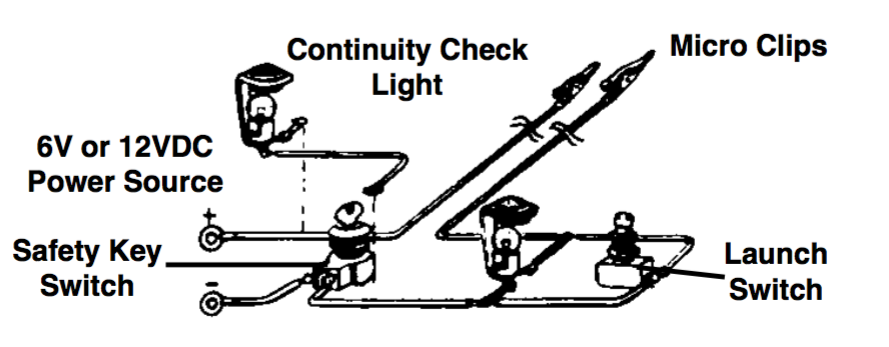
\includegraphics[width=10cm]{./images/fulcrum.png}
		\caption{Fulcrum model of perturbing forces on a model rocket}
		\label{fig:fulcrum}
	\end{figure}

	The rule of thumb provided by most model rocket makers and experts is that the CP should be at around 1 to 1.5 calibres (a calibre is equal to the diameter of the body tube) aft of the CG in order for the fins to have enough torque on the rocket body to stabilize the rocket during flight\cite{estes_rocket_tech} \cite{centuri_manual}. This number is called the stability margin. If it is below 1, then the fins may not have enough torque to overcome the perturbation. However if the margin is too large, then the fins begin to overcompensate for the perturbations and the rocket will exhibit ``weathercocking" which is seen as the the rocket oscillating back and forth during the flight which can significantly effect its apogee since energy from the thrust is diminished by the air drag rocking the rocket back and forth.

	In addition to taking care in positioning the CP sufficiently aft of the CM, it is also important to make sure that the CP and CM are aligned in the radial center of the rocket, so that there is no inherent torque on the rocket from airflow coming down from the nose of the rocket even at zero wind conditions.

	The basic overview of model rocketry mechanics provided above is sufficient to gain an understanding of the design decisions made in the report. Next up will be a brief introduction on model rocket telemetry, the remote collection  of data from the rocket that describes the its flight.

	\subsubsection{Model Rocket Telemetry}
	Rocket telemetry is at the heart of what makes many rocket enthusiasts keep coming back to launch their rockets over and over again. By being able to remotely retrieve flight data such as altitude, velocity, and acceleration from the rocket, rocket enthusiasts can get insight into their rocket's performance so that they can iterate and improve on their design. The most basic model rockets have no electronics inside, and the only way to approximate how high it went is use some clunky hand tools and trigonometery. Many technically inclined rocketeers and some companies build custom telemetry modules with altimeters and accelerometers on-board and a custom megahertz radio (very long range and simpler circuit design at lower frequecies compared to 2.4 GHz) for communication with a custom base station that collects the data from the rocket. The issue with custom telemetry modules is that it is not interoperable with other devices. In other words, to communicate with the telemetry module, one would need a custom base station with a custom radio on the same frequency as the one in the rocket, as opposed to just using a ubiquitous smartphone with a BLE chip already inside and a nice user interface in the form of an app. So to simplify the user experience and make telemetry more robust, a standardized and ubiquitous protocol such as BLE can be implemented for mid-ranged rocket telemetry.

\subsection{Bluetooth Low Energy}
	Bluetooth Low Energy (BLE) is a short range , ultra-low power, 2.4 GHz wireless communication protocol that has seen its rise to dominance thanks to the fast adoption of all major smartphone makers like Apple and Samsung, because of BLE's ability to extend the battery life of mobile devices with its ulta-low power consumption \cite{k_townsend_ble}. Its widespread adoptance with smartphone makers makes it espeically popular for ``smart" gadgets - consumer hardware products that can communicate with and be accessed from a smartphone. Notable examples include activity trackers like Fitbit, thermostats like Nest, and lightbulbs like Philips Hue. Because the protocol is highly standardized and designed to be low-cost and low-complexity, it makes it very easy for hardware developers to implement this protocol and very easy for consumers to use the product via a simple user interface on the smartphone. However, one major limitation to BLE is its range. Usually BLE devices are designed to operate within 50 meters of the user in order to extend battery life by operating the radio at very low power. In addtition, there is limitation in place from the Bluetooth Special Interest Group (SIG), who standardizes the specification for the BLE protocol, on the maximum radio broadcast powe which effectively limits the range to 100 meters \cite{k_townsend_ble}. This limitation significantly reduces BLE's application in mid-range toys like RC cars, quadcopter, and planes which often go upwards of 400 to 500 meters. Fortunately, the upcoming Bluetooth 5.0 specification in early 2017 will quadruple the range of BLE to roughly 400 meters while maintaining similar energy performance and thus immediately making the protocol an attractive option for toy makers.

	Thusly, in anticipation for the upcoming range increase of BLE and higher interest from toy makers, a model rocket reference design will be created to showcase the possibilities of a mid-range application of BLE.

\section{Design Requirements}

	The design requirements for this BLE model rocket reference design are basic and straight forward since it is a proof of concept (under limited development time of 3.5 months) to showcase the usage of BLE in mid-ranged toys such as a rocket, but it should have the features that take advantage of BLE to simply the user experience of launching rockets and yet make it more engaging. The design requirements for this PoC are the following:

	\begin{enumerate}
	\item Mechanical structure is constructed via 3D Printing
  \item Remote ignition of the rocket from the smartphone without an ignition box
	\item Maintain BLE communication with the rocket for at least 200 meters
	\item Flight minimum altitude of 150 meters (outside of typical BLE range)
	\item Communicate real-time altitude data to the smartphone
	\item Parachute can be ejected via a timer that can be configured from the smartphone before flight
	\item Parachute can be ejected via a remote command from the smartphone during flight
	\item Rocket can be recovered and reused multiple times
	\end{enumerate}

	Each item on the list can be broken down into very specific functional requirements in order to achieve those goals, and the majority of the rest of the report will be used to dissect how each design requirement is met both qualitatively and quantitatively.

	\subsection{Mechanical design is realized via 3D Printing}
	3D Printing is a rapid protoyping method to create mechanical structures orders of magnitude faster than machine shops and plastics molders and it is perfect for prototyping PoCs. This design requirement allows very quick iterations and experimentations of parts and assemblies within 2 days and is essential to completing this project on time. The mechanical design is done on a cloud-based Computer Aided Drawing (CAD) tool called OnShape and the file can be outputed directly to a 3D printer for printing. This subsection will discuss a few notable mechanical designs that were significant to the success of this project.

	





% The \ref{reference} command will create a reference to any \label command.
Here's a reference to table \ref{tbl:exampletable}

% The table environment is used to create a table. Note that by calling this environment,
% this table will automatically be added to the list of tables.
\begin{table}

	% The \centering command centres the table.
	\centering

	% The tabular environment creates the table itself. For more information
	% and options when using this environment, refer to the link under Tables provided
	% in README.md.
	\begin{tabular}{|c|c|c|} \hline
		title & number & decimal \\ \hline
		heading & 1 & 1.7 \\ \hline
		another heading & 2 & 3.4 \\ \hline
	\end{tabular}
	% The \caption{title} command adds a caption to your table. This caption will then
	% be used in the list of tables.
	\caption{A table demonstrating \LaTeX \, formatting}

	% The \label{title} command creates a reference that can be used to refer to this
	% table in the document. An example of this can be found on line 174.
	\label{tbl:exampletable}

\end{table}

\section{Math}

	\lipsum[1]

\subsection{The Bloch Equations}

	% The align environment is an important environment when writing out multiple
	% mathematical equations. It is used when vertical alignment is desired. Usually
	% binary relations, such as equal signs, are aligned.
	\begin{align}
		% The following are mathematical equations written using the amsmath
		% package. For more information on writing mathematical equations in
		% LaTeX, refer to the link under AMSMath in README.md.
		\frac{d\, M_x(t)}{dt} &= \gamma(\mathbf{M}(t) \times \mathbf{B}(t))_x - \frac{M_x(t)}{T_2} \\
		\frac{d\, M_y(t)}{dt} &= \gamma(\mathbf{M}(t) \times \mathbf{B}(t))_y - \frac{M_y(t)}{T_2} \\
		\frac{d\, M_z(t)}{dt} &= \gamma(\mathbf{M}(t) \times \mathbf{B}(t))_z - \frac{M_z(t) - M_0}{T_1}
	\end{align}

\subsection{The Schrodinger Equation}

	% The equation environment is used when only one equation needs to be written.
	\begin{equation}
		i\hbar \frac{\partial \, \Psi}{\partial t} = \hat{H}\Psi
	\end{equation}

\section{Graphics}

	Here's a stock image of a computer. It comes with a CC0 license, enabling
	free distribution for commercial and personal use. It's a JPEG.

	% The figure environment allows for the insertion of a figure into a LaTeX
	% document. By creating this environment, the figure will be automatically be added
	% to the list of figures. For more information on inserting figures, refer to the link
	% under Figures in README.md.
	\begin{figure}[!ht]
		\centering
		\label{fig:stock_computer}
		
\includegraphics[width=5cm]{./images/stock-image.jpg}
		\caption{A stock computer, I just wanted a picture here}
	\end{figure}

\section{Conclusions}

	% The \gls{title} command allows the LaTeX document to keep track of where words
	% in the glossary are used. For more information on the glossary and acronyms,
	% refer to the link under Glossary and Acronyms in README.md.
	\gls{LaTeX} is awesome.

\section{Recommendations}

	Use more \LaTeX. Also, use more \gls{Unix}. Also, citations like
    	\cite{k_townsend_ble} will lead to a better quality of work.

\end{body}


%%%%%%%%%%%
%  BACK MATTER  %
%%%%%%%%%%%

% The \begin{backmatter} command will create the backmatter environment. This
% environment includes the formatting required for the body, as well as the the

% backmatter environment. This environment is where the glossary, references, and appendices are inserted. You, the user, don't have to worry about inserting references or glossaries. These are built for you at compile-time from the \cite and \gls flags that you placed in your code, as well as entries in your bib files. The glossary and references are pre-pended to the appendices as separate pages at the beginning of this environment. You, however, must write your appendices in this environment.
\begin{backmatter}

% The appendix environment creates an appendix that will be properly added to
% table of contents. All figures and tables will be properly formatted to include the
% appendix letter.
\begin{appendix}{Here's An Appendix}

	\lipsum[1-2]

\end{appendix}

\begin{appendix}{Here's Another Appendix}

	\lipsum[1-2]

\end{appendix}

\begin{appendix}{A Figure in An Appendix}

	\lipsum[1-2]

	% This figure shows proper appendix formatting.
	\begin{figure}[!ht]
		\centering
		
\includegraphics[width=5cm]{./images/stock-image.jpg}
		\caption{It's back!}
	\end{figure}

	\begin{figure}[!ht]
		\centering
		
\includegraphics[width=5cm]{./images/stock-image.jpg}
		\caption{Testing Number}
	\end{figure}

\end{appendix}

\begin{appendix}{A Table in An Appendix}

        \lipsum[1-2]

	% This table shows proper appendix formatting.
        \begin{table}
		\centering

		\begin{tabular}{|c|c|} \hline
			\textbf{Abbreviation} & \textbf{Definition} \\ \hline
			BLE & Bluetooth Low Energy \\ \hline
			SoC & System on Chip \\ \hline
		\end{tabular}

		\caption{A Table in an Appendix, displaying the correct numbering}
        \end{table}

	\begin{table}
		\centering
		\begin{tabular}{|c|c|c|} \hline
			\textbf{Data} & \textbf{Integer} & \textbf{String} \\ \hline
			Foo & 1 & "bar" \\ \hline
		\end{tabular}
		\caption{Another table to test numbering}
	\end{table}

\end{appendix}

\end{backmatter}

\end{document}
